\section{Database}\label{sec:database}

\textbf{Authoriship: } Written by Nico Tasche\\
\emph{Minor proofreading \& edited by Andres Ardila} \\

\vspace*{4mm}

\subsection{Overview}\label{overview}

The chapter is all about how the collected data is stored and the API to
access the database. The focus is going to be database, the requirement,
decision making, architecture and data model. The API handles mainly the
access to the database and implements some optimizations mentioned in
the database article.

\subsection{Requirements}\label{requirements}

\subsubsection{Primary Requirements}\label{primary-requirements}

\begin{itemize}
\tightlist
\item
  scalable in the range of petabyte in size
\item
  hundreds of thousands of requests per minute
\item
  highly available
\item
  partition tolerant
\item
  fast to handle time-series
\item
  fast to handle geolocation data
\item
  immediate consistency is NOT necessary
\end{itemize}

As seen in the requirements, a huge focus was on scalability. We had
some secondary requirements as well, which were mainly regarding our
possibilities to handle the project.

\subsubsection{Secondary Requirements}\label{secondary-requirements}

\begin{itemize}
\tightlist
\item
  Open source or at the very least an open license is required.
\item
  must be well documented
\item
  must be manageable regarding administration and learning afford
\end{itemize}

\subsection{Survey of Existing
Solutions}\label{survey-of-existing-solutions}

Based on our knowledge, any relational database as main data storage has
been quickly disregarded. Fairly bad scaling behavior with the amount of
data we should be able to handle and the fixed data-schema architecture
were not a good fit for our use case. That does not mean, that a
relational database might be used for some special requirements.

Based on the preexisting experience in the group we had a closer look at
Elasticsearch and checked it against our requirements. This first look
was very promising, but more on that in the next chapter.

Other solutions in the realm of NoSQL databases were mainly web
research. That included what is out there and what is the strength and
weaknesses of each solution. That included mainly the big known ones
like Cassandra, MangoDB, \ldots{}

The survey of other existing NoSQL database solutions was not very
extensive, regarding real tests and in deep research. Because of the
feedback, which suggested we use the wrong database, we decided in the
middle of the project, to have an extra look at Apache Cassandra.

\subsection{Evaluation Criteria \& Decision-making
Process}\label{evaluation-criteria-decision-making-process}

The process of deciding what database architecture to use we started
with our requirements.

Besides the previously mentioned requirements we had some
soft-requirements as well:

\begin{enumerate}
\def\labelenumi{\arabic{enumi}.}
\tightlist
\item
  spread of database system
\item
  liveliness regarding
\item
  what was already known in the group
\end{enumerate}

\subsubsection{Why Elasticsearch}\label{why-elasticsearch}

Checking our requirements Elasticsearch fulfilled all of them. The
reasons why we decided to use Elasticsearch even before we went to deep
into other databases were as follows: - native support for geo spatial
searches \cite{McCandless.2016} - group members already knew Elasticsearch,
unlike all other NoSQL databases - extremely well documented - very high
development pace from the company who develops it

Considering we had no real database expert in our team, the fact that
group members already had practical experience with Elasticsearch was a
very important point for us.

\subsubsection{Special look at Cassandra}\label{special-look-at-cassandra}

After a few tests and an overview of the documentation, it was clear
that Cassandra had two shortcomings regarding our project. First, the
documentation seems to have quite a few gaps \cite{cassandra, cassandra2}. Second, there is no native support for spatial geo data.

\subsection{Implementation Details}\label{implementation-details}

\subsubsection{Intro to Elasticsearch}\label{intro-to-elasticsearch}

Elasticsearch \cite{eastic} is an open source Lucene based search
engine. It is under active development, with an extensive documentation.

\subsubsection{Architecture}\label{architecture}

Elasticsearch is a document store and works with indices, which are
comparable to tables in the classic SQL world. Each index holds JSON
based document which follow a mapping. The mapping is flexible and can
be extended however you want, but as soon as a field in the document has
a mapping, all documents with the same field have to follow that
mapping. E.g. if a document has a field called location, which is mapped
to a geopoint data type. Every document with a field name location, must
have a geopoint in it.

Each index can be sharded and each node/server-instance can have
multiple indices. To better distribute search requests, the workload is
divided among all shards belonging to an index and means that each shard
holds just one part of an index. Because that would not scale very well
and would have no partition tolerance, each index has a configurable
number of replicas. A new search request is send to one replica of each
shard.

Elasticsearch automatically handles the distribution of search requests
to the primary shards or replicas. Depending on the number nodes in a
Elasticsearch cluster, the engine also automatically distributes the
shards and replicas to the different nodes, all according to the
configuration made for each index. To illustrate that see the following
figure, which assumes that the cluster holds three indices, on three
nodes, with two replicas per index.

\begin{figure}[htbp]
	\centering
	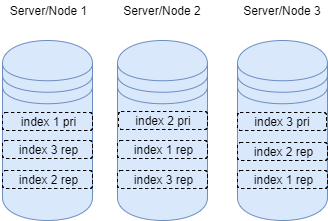
\includegraphics[width=0.7\textwidth]{images/07_database_architecture_elastic.png}
	\caption{OpenData Database Architecture}
	\label{fig:elastic-architecture}
\end{figure}

The index configuration in our architecture follows a template, which is
automatically applied to each new index we create:

\begin{verbatim}
{
  "template": "data-*",
  "order": 1,
  "settings": {
    "number_of_shards": 1,
    "number_of_replicas": 3
},
"mappings": {
  "_default_": {
    "_all": {
      "enabled": false
    }
  },
  "data": {
    "properties": {
      "device": {
        "type": "keyword"
      },
      "location": {
        "type": "geo_point"
      },
      "timestamp": {
        "type": "date"
      },
      "timestamp_record": {
        "type": "date"
      },
      "license": {
        "type": "text"
      }
    }
  }
}
\end{verbatim}

This template provides the number of shard, replicas and the basic
mapping for our data model. If necessary this information can be
overwritten before a new index is created. This is all the necessary
information needed for our architecture and cannot be changed after an
index is created, except for the number of replicas, which can be
increased.

\subsubsection{Data Model}\label{data-model}

We decided to have a data model which is data-source-centric with the
extra possibility to partition the data over time. That means, each data
source gets its own index with its own timeframe and its own adjusted
data structure. All our data sources save a few basic data points with
each element stored in the database, in particular are those: -
\texttt{timestamp}: when has the data point been recorded -
\texttt{location}: where has the data point been recorded

Those are the only information we need to store, besides the individual
measurements. We do actually store some more information, but regarding
the common use cases for searches those two data points are enough for
environmental data. For each data entry then, there are one ore many
measurements in that data point. Each measurement than has a quality
indicator, a observed value and an sensor name. Please refer to the full
data-model in the project wiki for more information.

There were mainly two reasons to use this data model. For one it keeps
the data provenance, which we quite like to keep. The second reason is
that it is nice to handle in terms of partitioning.

\subsubsection{Partitioning}\label{partitioning}

As for the question, how does the used data model scale and how to best
partition the imported data we decided for a 2-dimensional approach. One
dimension is already covert by the data-source centric data model, which
allows us, to partitioning by source. The second dimension is the time.
Each data source is partitioned based on the time a measurement has been
taken and the granularity can be adjusted as well.

This gives us multiple advantages:

\begin{itemize}
\tightlist
\item
  it allows us to adjust the server infrastructure based on the data
  source
\item
  it scales indefinitely
\item
  index size is deterministic, because of time based partitioning
\end{itemize}

So why does it scale so good? When importing data from one source, I
process and store the data points in one index. This index is not just
limited to the data source, it is also limited to the time, e.g.~2016.
That means, when 2016 is finished with importing data, the index is done
and can be closed up, no one needs to care about it anymore. After the
index is done, it might even be transferred to another Elasticsearch
node with different hardware. That would be useful, for example, when
the average density of the smurf population is being stored. The index
can be transferred to a less powerful hardware with fewer CPU cores and
spinning hard drives and even fewer replicas, because this information
is probably hardly requested, except from Gargamel and maybe some surf
protection groups.

As a starting point, we choose to configure each index as shown in the
figure below. We decided to keep each index on one shard, which lowers
the network traffic and because we are very flexible regarding the size
of the index thanks to our time-based partitioning, this should not
become a problem later on. To allow thousands of request per second, we
decided to start with three replicas, so each request is forwarded to a
different replica. This can be flexible in- or decreased later on.

\begin{figure}[htbp]
	\centering
	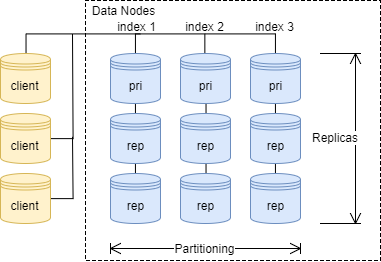
\includegraphics[width=0.8\textwidth]{images/07_database_architecture.png}
	\caption{OpenData Database Architecture}
	\label{fig:db-architecture}
\end{figure}

\subsubsection{Query Optimization}\label{query-optimization}

Why do we need query optimization? For that I'm going to give a small
example to consider:

\begin{enumerate}
\def\labelenumi{\arabic{enumi}.}
\tightlist
\item
  we import multiple sources, with multiple measurements:
  source1(air-temperature, water-temperature) 1980 - 2017,
  source2(air-temperature) 1983 - 1990, source3(uv-index) 2009 - 2017
\item
  each source is partitioned by year and source 1 is partitioned by
  month for all data after 2015.
\item
  every index is naively sharded over 3 nodes (we actually use just one
  shard per index)
\end{enumerate}

Let's make a simple search request: give me all UV values data from 2015
till 2017 and aggregate an average over the month. Because the user does
not know anything about the internal database architecture (at least he
should not) he requests the temperature and the timeframe.

\textbf{Worst case:}

A search request in send to all indices, that means:

\begin{verbatim}
source1 = 35 years + (2years x 12 month) x 3 shards
source1 = 177 shards

source2 = 17 years x 3 shars
source2 = 51 shards

source3 = 8 years x 3 shars
source3 = 8 years x 3 shars

source1 + source2 + source3 = 252 shards
\end{verbatim}

So in worst case each shard has its own node(very unlikely), the search
request has to be send to 252 nodes/computers.

\textbf{First optimization: Limit the time}

With a naive approach by checking the common time part of the request
2016-2017 and limit the indices search with the following pattern:

\begin{verbatim}
indexsearch: *-201*
\end{verbatim}

\begin{verbatim}
source1 = 5 years + (2years x 12 month) x 3 shards
source1 = 87 shards

source2 = 0 years x 3 shars
source2 = 0 shards

source3 = 3 years x 3 shars
source3 = 9 shards

source1 + source2 + source3 = 96 shards
\end{verbatim}

We already reduced the number of shards we need to address by 61\%

With a little more sophisticated time limitation algorithm, we could
actually do more and search just those two years:

\begin{verbatim}
indexsearch: *-2016, *-2017
\end{verbatim}

\begin{verbatim}
source1 = 1 years + (2years x 12 month) x 3 shards
source1 = 75 shards

source2 = 0 shards

source3 = 2 years x 3 shards
source3 = 6 shards

source1 + source2 + source3 = 81 shards
\end{verbatim}

Now we are at 68\% reduction.

\textbf{Second optimization: Limit to indices which contain the right
data}

If we store in a separate database, which data source and therefore
indices actually hold the requested data we can do even much more:

\begin{verbatim}
indexsearch: source3-2016, source3-2017
\end{verbatim}

\begin{verbatim}
source1 = 0
source2 = 0 shards
source3 = 2 years x 3 shards = 6 shards

source1 + source2 + source3 = 6 shards
\end{verbatim}

By using those two optimizations, we could reduce the number of
requested shard to 6, which means a total reduction of 96.2\%.

This was just a naive example. The reduction should even be much higher
in a production environment, with a growing number of data sources.
Let's say we have already 100 data sources and we can limit a request to
just two of those for example because the requested measurement it
provided just by those two, the saving of network traffic and workload
would be immense.

\subsection{API Implementation
Details}\label{api-implementation-details}

\subsubsection{Overview}\label{overview-1}

As for the API, it was important for us to provide a solution which is
easy to scale via a load balancing, for example with an nginx instance
as an entry point for the user of our system. That means, those
instances need to be stateless. For that and because it is basically a
standard we use a REST interface to provide access to our
data-collection.

\subsubsection{Architecture and
Technology}\label{architecture-and-technology}

As base technology, we use NodeJS, which is easy to use JavaScript
runtime based on Chrome's V8 JavaScript engine. It allows a fast
iteration pace and needs just minimal preparation to develop server
instances with.

\begin{figure}[htbp]
\centering
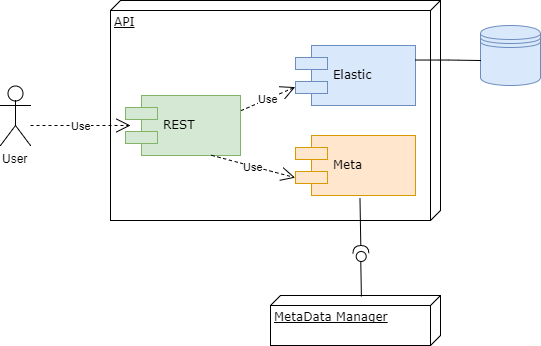
\includegraphics[width=1.00\textwidth]{images/07_API_Architecture.png}
\caption{Public API Abstraction}
\label{fig:public-api}
\end{figure}

The API implementation consists of three parts.

\begin{enumerate}
\def\labelenumi{\arabic{enumi}.}
\tightlist
\item
  Route: defines all routes and parses all parameters to be used in our
  system
\item
  Meta: connects to the management database and requests all necessary
  data (this part is prepared, but connection not implemented yet)
\item
  elastic: does everything Elasticsearch specific and could be replaced
  by another database connection if the database would be replaced for
  example.
\end{enumerate}

\subsubsection{REST APIs}\label{rest-apis}

The REST API currently consists of three endpoints:

\textbf{1. GET /api/sources/}

Returns all currently available resources

\textbf{2. GET /api/sources/:indexName}

Returns data based on the sources they came from

\textbf{3. GET /api/measurements/:measurements}

Returns data based on the measurements you're requesting

The 2nd as well as the 3rd REST-endpoint allow a more specific search,
based on extra parameters.

\textbf{Parameters:}

\begin{figure}[htbp]
\centering
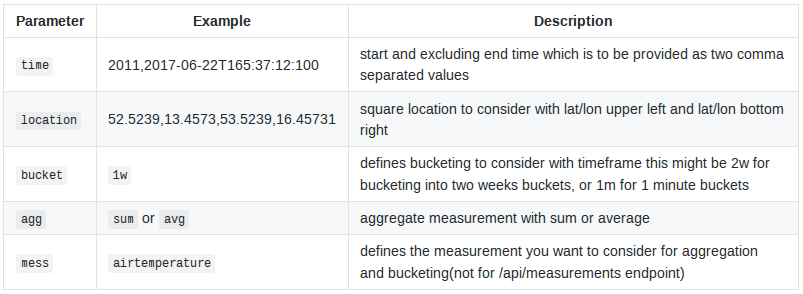
\includegraphics[width=1.00\textwidth]{images/07-table.png}
\end{figure}

\subsection{Discussion}\label{discussion}

\subsubsection{Joins}\label{joins}

One mayor drawback of Elasticsearch is the missing possibility of
server-side join, the way they are known by SQL based database-system.
This means, any kind of join operation must be done either on a separate
server, like our API instance, or on the application side. This is
something we were not aware of for quite a long time.

\subsubsection{Administration}\label{administration}

This is probably not a Elasticsearch specific but should be mentioned in
this chapter as well. To setup this the basic database is quite easy,
but to scale it to up to petabyte needs quite a bit consideration. Our
data model and the current implemented optimizations will help scale the
database and everything should work without any performance drawbacks
for quite a while. To archive this, lots of working though documentation
and local request testing had to be done. As said before, this is
probably for every other database as well.

\subsubsection{Testing}\label{testing}

Testing is something we could just do on a very limited scale.
Unfortunately, any possible short-comings in our architecture would just
show much later then we could test.

\subsection{Future Development and
Enhancements}\label{future-development-and-enhancements}

\subsubsection{Data Postprocessing}\label{data-postprocessing}

As mentioned in the Limitations section, joins are not possible in our
system right now. One way of doing it would be to allow application
based or backend based join, which will have same limitations. A better
way would be to post process our data at low usage times. One idea would
be to collect all the data for a defined area and put all information we
have about that area into one dataset. The area could be for example a
size of 100m x 100m. This would allow for very fast, very complex
queries, which involves quite a few measurements.

\subsubsection{The API}\label{the-api}

The current implementation of the API is somewhat limited. This is
mainly due to time limitations while implementing. These are the points,
which should be implemented:

\begin{enumerate}
\def\labelenumi{\arabic{enumi}.}
\tightlist
\item
  Allowing to make post requests to make more complex queries. That
  would for example include the transfer of big geospatial shapes for
  filtering.
\item
  Adding security with API tokens
\item
  Adding full access to the management database
\item
  Adding safety checks like timeouts to make not to extensive requests
\item
  Adding possibility for scrolling to request data in chunks
\item
  optimizing the data handling on the API instances, which is not very
  efficient
\end{enumerate}